\chapter{Конструкторский раздел}

В данном разделе будут рассмотрены требования к программе и алгоритмы визуализации сцены и молнии.


\section{Общий алгоритм решения поставленной задачи}
\begin{enumerate}
	\item Задать объекты сцены (цилиндр, жидкость, стержень).
	\item Разместить источник света.
	\item С помощью обратной трассировки лучей визуализировать обстановку.
\end{enumerate}


\section{Алгоритм обратной трассировки лучей}


Алгоритмы трассировки лучей на сегодняшний день считаются наиболее приближен к реальности при создании изображений. 

Изображение формируется за счет того, что отраженный свет попадает в камеру. Выпускается множество лучей (первичные) из источников света. Часть этих лучей “улетает” в свободное пространство, а часть попадает на объекты сцены, преломляясь и отражаясь, при том часть энергии лучей поглощается в зависимости от физических свойств материала объекта. 

Преломленные и отраженные лучи продолжают взыскиваться до предела выставленным в программе. В конечном счете часть лучей попадает в камеру и формирует изображение.
Данный алгоритм называется прямой трассировкой лучей, но он крайне неэффективен, так как большинство лучей, исходящих из источника света, не попадают в камеру. 
Оптимизированный алгоритм трассировки лучей называется обратный. 
В данном алгоритме лучи отслеживаются из камеры, а не из источников света. Таким образом, программно обрабатывается меньшее количество лучей.

Предполагается, что есть камера и экран (рисунок \ref{img:tracric}), находящийся на определенном расстоянии от нее. Экран разбивается на пиксели, далее поочередно испускаются лучи из камеры в центр каждого пиксела. Находится пересечение каждого луча с объектами сцены и выбирается среди всех пересечении наиболее близкое к камере. Далее, применяется модель освещения и получается изображение сцены. Это самый простой метод трассировки лучей, который отсекает невидимые грани.


\begin{figure}[ht!]
	\begin{center}
		\captionsetup{singlelinecheck = false, justification=centerfirst}
		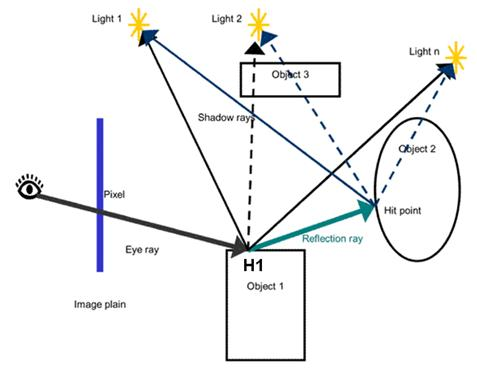
\includegraphics[scale=0.8]{assets/tracric.jpeg}
		\caption{Пример работы алгоритма обратной трассировки лучей}
		\label{img:tracric}
	\end{center}
	
\end{figure}


В усложненном алгоритме учитывается отражение, для этого необходимо из самого близкого пересечения пустить вторичные лучи.

На рисунке \eqref{fig:ref3} представлена схема алгоритма.

\begin{figure}[ht!]
	\centering{
		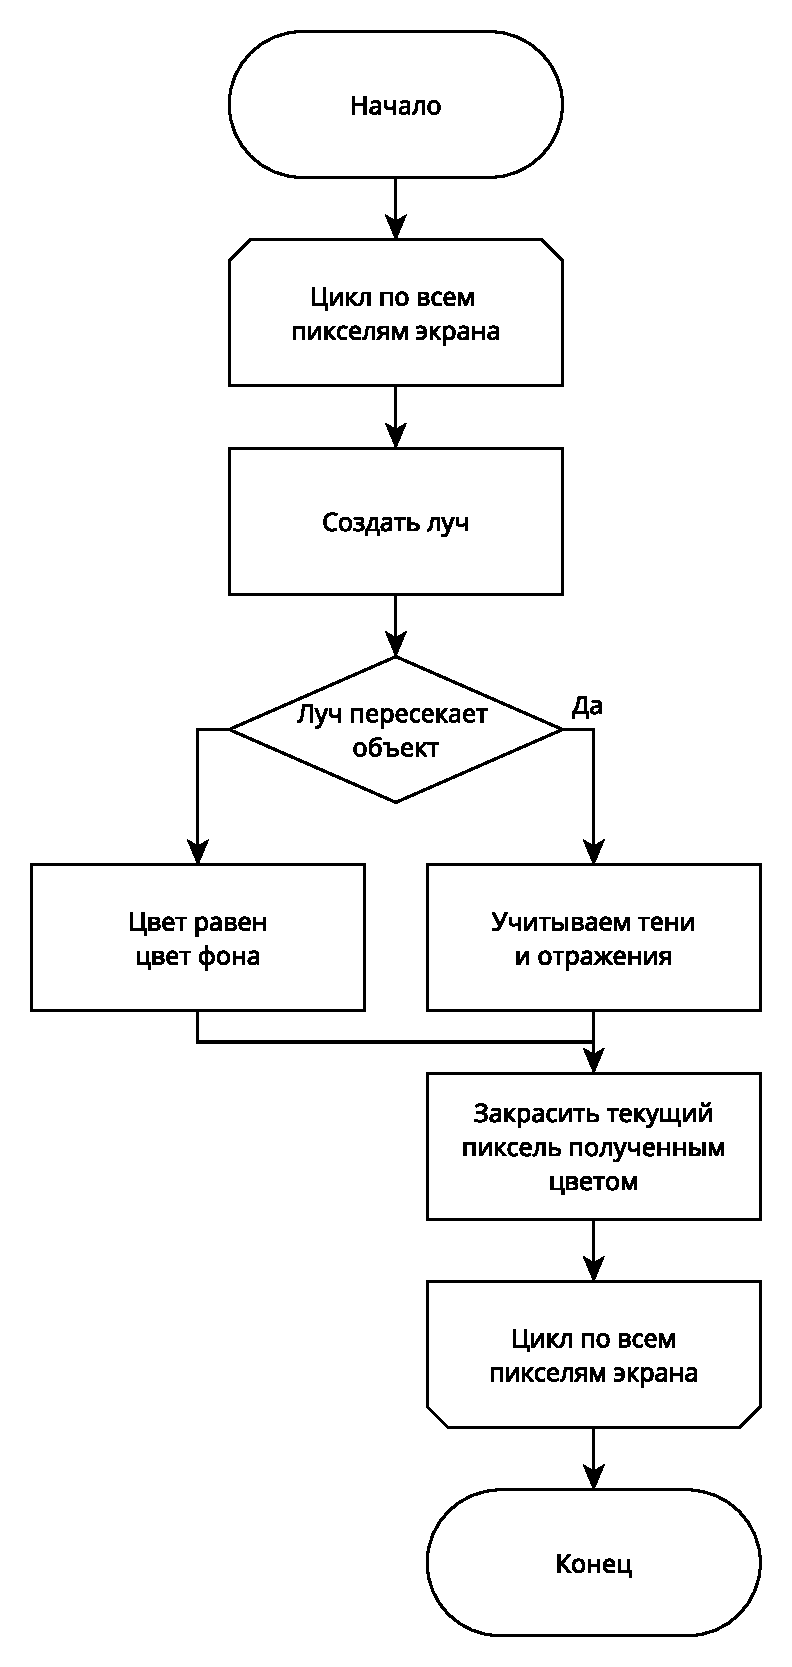
\includegraphics[width=0.6\textwidth]{assets/trace-alg.pdf}
		\caption{Cхема алгоритма трассировки лучей}
		\label{fig:ref3}}
\end{figure}

\newpage

\section{Алгоритм преломления лучей в прозрачных объектах}

Чтобы изобразить прозрачный объект, в его материале должны задаваться отражение и преломление (рисунок \ref{img:lomka}). 

Если поверхность обладает отражающими свойствами, то строится вторичный луч отражения. Направление луча определяется по закону отражения (геометрическая оптика) равна 

$r = i - 2 \cdot n \cdot (n \cdot i)$.

\begin{figure}[ht!]
	\begin{center}
		\captionsetup{singlelinecheck = false, justification=centerfirst}
		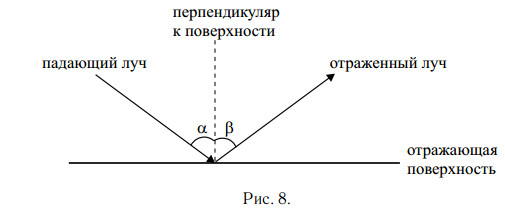
\includegraphics[scale=1]{assets/lomka.jpeg}
		\caption{Направление луча по закону отражения}
		\label{img:lomka}
	\end{center}
	
\end{figure}

Если же поверхность прозрачна, то строится луч прозрачности. Для определения направления луча используется закон преломления (рисунок \ref{img:lomka-2}).

\begin{figure}[ht!]
	\begin{center}
		\captionsetup{singlelinecheck = false, justification=centerfirst}
		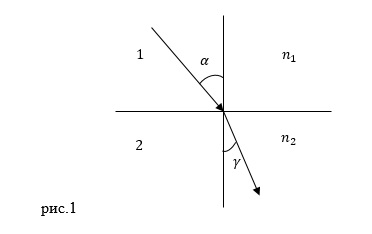
\includegraphics[scale=1]{assets/lomka-2.jpeg}
		\caption{Направление луча по закону преломления}
		\label{img:lomka-2}
	\end{center}
	
\end{figure}

\section{Модель освещения Фонга}

Наиболее распространенная модель в обратной трассировке лучей эмпирическая модель - освещения по Фонгу. Данная модель вычисляет цвет поверхности в зависимости от того как на нее светит источник света, а также от поверхности самого объекта. Согласно данной модели, освещенность точки равна 
\begin{equation}
	C_{out} = C \cdot (k_a + k_d \cdot max(0, (n\cdot I)) + I \cdot k_s \cdot max(0, v \cdot (v \cdot r)^p))
\end{equation}


\section{Пересечения луча и сферы}

Уравнение луча представлено ниже:

\begin{equation}
	P = O + t(V - O), t \geq 0,
	\label{eq:ref5}
\end{equation}
где О - центр камеры, а V - текущий пиксель.

Обозначим направление луча:

\begin{equation}
	\overrightarrow{D} = V - O
\end{equation}

Уравнение \eqref{eq:ref5_1} эквивалентно уравнению \eqref{eq:ref5}.

\begin{equation}
	{\begin{cases}
			x(t) = x_O + t x_D \\
			y(t) = y_O + t y_D \\
			z(t) = z_O + t z_D
			\label{eq:ref5_1}
	\end{cases}}
\end{equation}

Рассмотрим, что собой представляет сфера.

%\begin{figure}[ht!]
%	\centering{
	%		\includegraphics[width=0.5\textwidth]{img/sphere.jpg}
	%		\caption{Сфера}}
%\end{figure}

Сфера — это множество точек P, лежащих на постоянном расстоянии r от фиксированной точки C. Тогда можно записать уравнение, удовлетворяющее этому условию:

\begin{equation}
	distance(P,C) = r
	\label{eq:ref6}
\end{equation}

Запишем расстояние (\ref{eq:ref6}) между P и C как длину вектора из P в C:

\begin{equation}
	|P-C|=r
\end{equation}

Заменим на скалярное произведение вектора на себя:

\begin{equation}
	\sqrt{\langle P - C\rangle, \langle P - C\rangle} = r
\end{equation}

Избавимся от корня:

\begin{equation}
	\langle P - C\rangle, \langle P - C\rangle = r^2
	\label{eq:ref7}
\end{equation}

В итоге есть два уравнения - уравнение луча и сферы. Найдем пересечение луча со сферой. Для этого подставим (\ref{eq:ref5}) в (\ref{eq:ref7})

\begin{equation}
	\langle O + t\overrightarrow{D} - C \rangle, \langle O + t\overrightarrow{D} - C\rangle = r^2
\end{equation}

Разложим скалярное произведение и преобразуем его. В результате получим:

\begin{equation}
	t^2 \langle \overrightarrow{D}, \overrightarrow{D} \rangle + 2t \langle \overrightarrow{OC}, \overrightarrow{D} \rangle + \langle \overrightarrow{OC}, \overrightarrow{OC} \rangle -r^2 = 0
	\label{eq:ref8}
\end{equation}

Представленное квадратное уравнение (\ref{eq:ref8}) имеет несколько возможнных случаев решения.
Если у уравнения одно решение, это обозначает, что луч касается сферы.
Два решения обозначают, то что луч входит в сферу и выходит из неё.
И если нет решений, значит, луч не пересекается со сферой.

\section{Пересечения луча и цилиндра}
Бесконечный цилиндр, образующие которого параллельны оси z, описывается уравнением\eqref{eq:ref9}.

\begin{equation}
	x^2 + y^2 = r^2
	\label{eq:ref9}
\end{equation}

Аналогичные уравнения \eqref{eq:ref10} и \eqref{eq:ref11} для
бесконечных цилиндров, образующие которых параллельны осям x и y соответственно.

\begin{equation}
	y^2 + z^2 = r^2
	\label{eq:ref10}
\end{equation}

\begin{equation}
	x^2 + z^2 = r^2
	\label{eq:ref11}
\end{equation}

Рассмотрим цилиндр, выровненный вдоль оси z (уравнение \ref{eq:ref9}).
Аналогичные решения получатся для \eqref{eq:ref10} и \eqref{eq:ref11}.
Найдем пересечение луча с цилиндром.
Для этого подставим \eqref{eq:ref5_1} в \eqref{eq:ref9}

\begin{equation}
	(x_O + t x_D)^2 + (y_O + t y_D)^2 = r^2
	\label{eq:ref12}
\end{equation}

Вынесем t из скобок в уравнение \eqref{eq:ref12} и получим \eqref{eq:ref13}.

\begin{equation}
	t^2(x_D^2+y_D^2) + 2t(x_Ox_D + y_Oy_D) + (x_O^2 + y_O^2 - r^2) = 0
	\label{eq:ref13}
\end{equation}

Решение представленного уравнения (\ref{eq:ref13}) можно получить решив дискриминант.
Уравнение (\ref{eq:ref13}) квадратное и имеет соответствующие случаи решения.


Для конечного цилиндра нужно ввести ограничение по оси.
Для цилиндра, записанного уравнением (\ref{eq:ref9}), данные ограничения
продемонстрированы в (\ref{eq:ref14}).

\begin{equation}
	z_{min} < z < z_{max}
	\label{eq:ref14}
\end{equation}

Получив $t_1$ и $t_2$ из уравнения (\ref{eq:ref13})
найдем $z_1$ и $z_2$ с помощью уравнения (\ref{eq:ref5_1}).
Далее необходимо произвести проверку (\ref{eq:ref15}).

\begin{equation}
	{\begin{cases}
			z_{min} < z_1 < z_{max} \\
			z_{min} < z_2 < z_{max}
			\label{eq:ref15}
	\end{cases}}
\end{equation}

Если обе точки проходят данный тест, то наименьшее неотрицательное
значение t -- это ближайшая точка пересечения луча с конечным цилиндром.

\section{Пересечения луча и параллелепипеда}

Задача (определить, пересекает ли луч какой-либо объект в трёхмерном пространстве). Параллелепипед задаётся координатами двух своих вершин: той, у которой все три координаты минимальны, и той, у которой все три координаты максимальны. 
Таким образом, мы сразу получаем шесть плоскостей, ограничивающих параллелепипед --- и все шесть параллельны координатным плоскостям (т.е. задаются в пространстве уравнениями вида x = a).

Для начала мы проверяем, не лежит ли начало луча внутри параллелепипеда. Если лежит, то ответ на вопрос о пересечении лучом параллелепипеда --- сразу положительный, более ничего проверять не надо. 
Если же начало луча лежит вне параллелепипеда --- тогда необходимо вычислить пересечение.

Если x-компонента направляющего вектора луча отлична от нуля, мы ищем параметры точек пересечения луча с теми двумя плоскостями, ограничивающими параллелепипед, которые перпендикулярны оси X. Это параметры $t_1$, $t_2$. 
Если оба параметра отрицательны --- значит, луч не пересекает эту пару плоскостей, т.е. не пересекает и параллелепипед. 

Если один неотрицательный --- тогда мы их записываем в переменные $t_{near}$, $t_{far}$. Если же x-компонента направляющего вектора луча равна нулю --- тогда нужно проверить, лежит ли x-компонента начальной точки луча между нашими двумя плоскостями, ограничивающими параллелепипед, которые перпендикулярны оси X. 
Если не лежит --- ответ сразу отрицательный, луч не пересекает параллелепипед. Для оставшихся двух пар плоскостей --- аналогично. И если в ходе мы нигде не получили отрицательный результат --- значит, он положительный.

\section{Выбор используемых типов и структур данных} 

Для разрабатываемого ПО необходимо реализовать следующие типы и структуры данных.
\begin{enumerate}
	
	\item Трехмерный вектор - хранит направление, задается координатами x, y, z.
	
	\item Цвет - вектор из трех чисел (синий, красный, зеленый).
	\item Сфера - хранит радиус, цвет, положение, коэффициент преломления, коэффициент отражения, эмиссию.
	\item Цилиндр - хранит радиус, высоту, цвет, положение, коэффициент преломления, коэффициент отражения, эмиссию.
	\item Поверхность - хранит высоту, цвет, положение, коэффициент преломления, коэффициент отражения, эмиссию.
	\item Прямоугольный параллелепипед - хранит цвет, положение, положение второй точки, коэффициент преломления, коэффициент отражения, эмиссию.
	\item Сцена - список объектов, камеру, источник света.
	\item Источник света - положение и направление света.
	\item Камера - положение.
	
\end{enumerate}


\section{Вывод}
В данном разделе были подробно рассмотрены алгоритмы, которые будут реализованы, и приведена схема алгоритма обратной трассировки лучей, указан способ оптимизации данного алгоритма для решения поставленной задачи и описаны используемые структуры.